\section{VideoQA Reformulation}
\label{sec:reformulation}

Discovering the grounding rationale for faithful prediction demands careful inspection of the data generating process. In favor of the causal theory \cite{pearl2016causal}, we review the formation of VideoQA models, then formalize them as a Structure Causal Model (SCM) \cite{alma991011292629705181}  by investigating causality among five variables: the input video $V$ and question $Q$, the causal scene $C$ and its environmental scene $E$, ground-truth answer $A$.

\subsection{Causal Graph of VideoQA}
Scrutinizing the relations among its variables, we abstract the formulation of VideoQA in Figure \ref{fig:scm}a and explain its rationality as follows:

\begin{itemize}[leftmargin=*]
    % \setlength\itemsep{-2pt}
    \item $Q\to C, E \gets V$. Given the semantic of question $Q$,  input video $V$ is composed of a question-critical scene $C$ and $E$--the uninformative part. For example, the video in Figure \ref{fig:overview} is consists of two green clips (\ie $C$) and one blue clip (\ie $E$).
    
    \item $V,Q\to C\to A$. Filtered by question clue, the distilled visual information $C$ contains answer-decisive knowledge that is sufficient to yield answer $A$.
    
    \item $V,Q\to A$. In addition to retrieving $C$, $V$ and $Q$ also deliver a uni-modal message to the classifier. Albeit the underlying bias in some analyses \cite{cadene2019rubi,niu2020counterfactual}, they disclose essential prior statics on the environment. 
    
    \item $E\dashleftarrow\dashrightarrow C$. The dashed arrow sketches adjunctive probabilistic dependencies \cite{reason:Pearl09a} between $C$ and $E$, which is typically rising from selection bias \cite{DBLP:conf/cvpr/TorralbaE11}. For example, the ``landscape'' of the video in Figure.\ref{fig:overview} is frequently collected as a common environment for the ``horse-riding '' scene. 
    
\end{itemize}
\subsection{Beyond ERM}

Inspecting previous efforts, we sketch the SCM for the conventional ERM-guided method in Figure \ref{fig:scm}b.  Probing its causal structure, we investigate the inability of the conventional method in locating the grounding rationale, which shed light on how EGV addresses the problem accordingly.
%
In conventional VideoQA, the $V, Q$ pair is directly paired together to model their interaction and then generates the $A$ as a prediction. Inevitably, such exploitation takes $V$ as a whole and ignores the data generation process, where $C$ and $E$ hold different attribution towards answer semantic. 
%
Driven by ERM, conventional methods blindly capture the statistical correlations between input $(V, Q)$ pairs and answers, while discarding the functional divergence of $C$ and $T$ in the reasoning logic. As a result, such brutal optimization is inept for intrinsic interpretation.

%, make the partition result venerable against environment shift (\ie even a permutation on complement can result in a drastic change on interpretation), and jeopardizes the inept for . 
    
% conventions methods dismiss the formation of $V$ and blindly captures the statistical correlations between input $(V, Q)$ pairs and answers, this makes themselves venerable against environment shift (\ie even a permutation on complement can result in a drastic change on interpretation), and inept for intrinsic interpretation.   
%
Intuitively, a hard split on question-relevant part $C$ naturally serves as the interpretation of the prediction. Following this essence, we present the insight of EGV (Figure \ref{fig:scm}c) by eliminating the effect of environment scene $E$. 
%
In fact, eradicating $E$ from reasoning logic makes $C$ the only component of the input video, thus cutting off  $V \to A$ and emphasizing the impact of $C \to A$.







\begin{figure}[t]
\centering
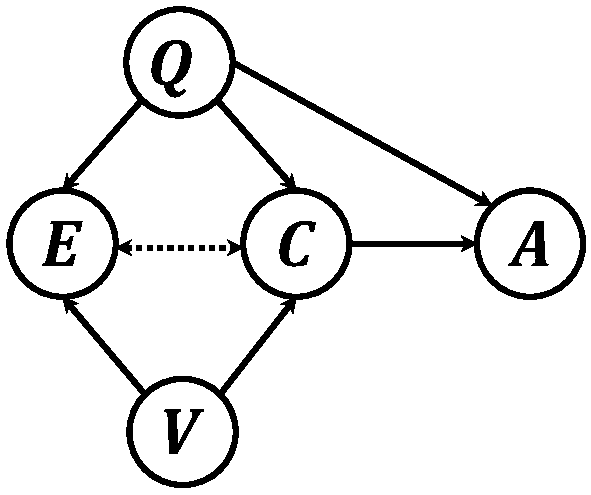
\includegraphics[scale=0.28]{fig/scm.pdf}
\caption{Causal Graph of VideoQA}
\vspace{-5pt}
\label{fig:scm}
\end{figure}
